\chapter{Godot}
\label{cap:godot}

Voltaremos nossa atenção à \textit{game engine} \textit{Godot} neste capítulo. Em particular, estamos interessados no estudo dos elementos principais que compõe sua arquitetura, a organização do seu código fonte e instruções para compilação.

Para referência, todas as informações relacionadas a \textit{Godot} são referentes à versão \textbf{2.1.4}, que é a mais recente e estável no momento de escrita deste trabalho.

Todas as instruções e comandos apresentados foram originalmente realizados no sistema \texttt{Ubuntu 16.04 LTS, 64-bit} do autor.

% ---------------------------------------------------------------------

\section{História}

O desenvolvimento de \textit{Godot} começou em 2007, através de Juan Linietsky e Ariel Manzur. O nome foi escolhido em homenagem à peça \emph{Waiting for Godot}, de Samuel Beckett, para representar uma biblioteca que cada vez mais ganha novas funcionalidades, mas nunca chegará a um produto definitivo \citep{godotHistory}.

\textit{Godot} é notavelmente conhecido por possuir código aberto, que foi liberado ao público em fevereiro de 2014. Desde então, ganha constantes atualizações para se equiparar a \textit{game engines} competidoras mais sofisticadas, como \textit{Unity} e \textit{Unreal Engine}. Atualmente, encontra-se na versão 2.1.4, com uma versão 3 em beta, e possui suporte para a produção de jogos em diversas plataformas, entre elas Unix, Windows, MacOS, Android, iOS e web.

% ---------------------------------------------------------------------

\section{Linguagens}

\textit{Godot} possui seu código fonte escrito primordialmente em \textbf{\textit{C++}}. Apesar de não possuir toda a versatilidade de uma linguagem de \textit{script} como \textit{Python} e \textit{Ruby}, um código escrito em \textit{C++} possui uma execução bem rápida, fator crítico para um software que produzirá jogos. Comparado ao antecessor, \textit{C}, a linguagem oferece ferramentas mais poderosas, como Orientação a Objetos e bibliotecas para tipos abstratos de dados (pilhas, filas, etc.).

Um usuário da \textit{game engine}, no entanto, raramente interage diretamente com \textit{C++}. Ao invés disso, usa-se uma interface gráfica, na forma de um editor, com várias facilidades para a criação de jogos. Para programação, \textit{Godot} disponibiliza uma linguagem de \textit{script} nativa chamada \mbox{\textbf{\textit{GDScript}}}.

\textit{GDScript} possui uma sintaxe extremamente simples, parecida com \textit{Python}, e foi projetada para usufruir da arquitetura da \textit{game engine}. O usuário pode programar classes, estruturas e partes de seu jogo com maior facilidade, utilizando as ferramentas oferecidas pelo software sem precisar se preocupar com detalhes internos de implementação \citep{godotGDScript}. Em outras palavras, \mbox{\textit{GDScript}} age como uma ``linguagem intermediária'' entre o usuário e as interfaces em \textit{C++} que \textit{Godot} disponibiliza.

% ---------------------------------------------------------------------

\section{Arquitetura}

A arquitetura de \textit{Godot} é bastante complexa, chegando a mais de 7 milhões de linhas de código. Uma análise criteriosa de todos os componentes fugiria do contexto deste trabalho. No entanto, é essencial entender as principais classes e conceitos da \textit{game engine} para podermos implementar, com sucesso, o módulo de reconhecimento de voz.

A título de curiosidade, uma árvore de herança de classes é mostrada na figura \ref{godotClasses}. Os filhos das classes \textit{Control}, \textit{Node2D}, \textit{Reference} e \textit{Spatial} foram omitidos por serem muito numerosos.

\begin{figure}[H]
  \centering
  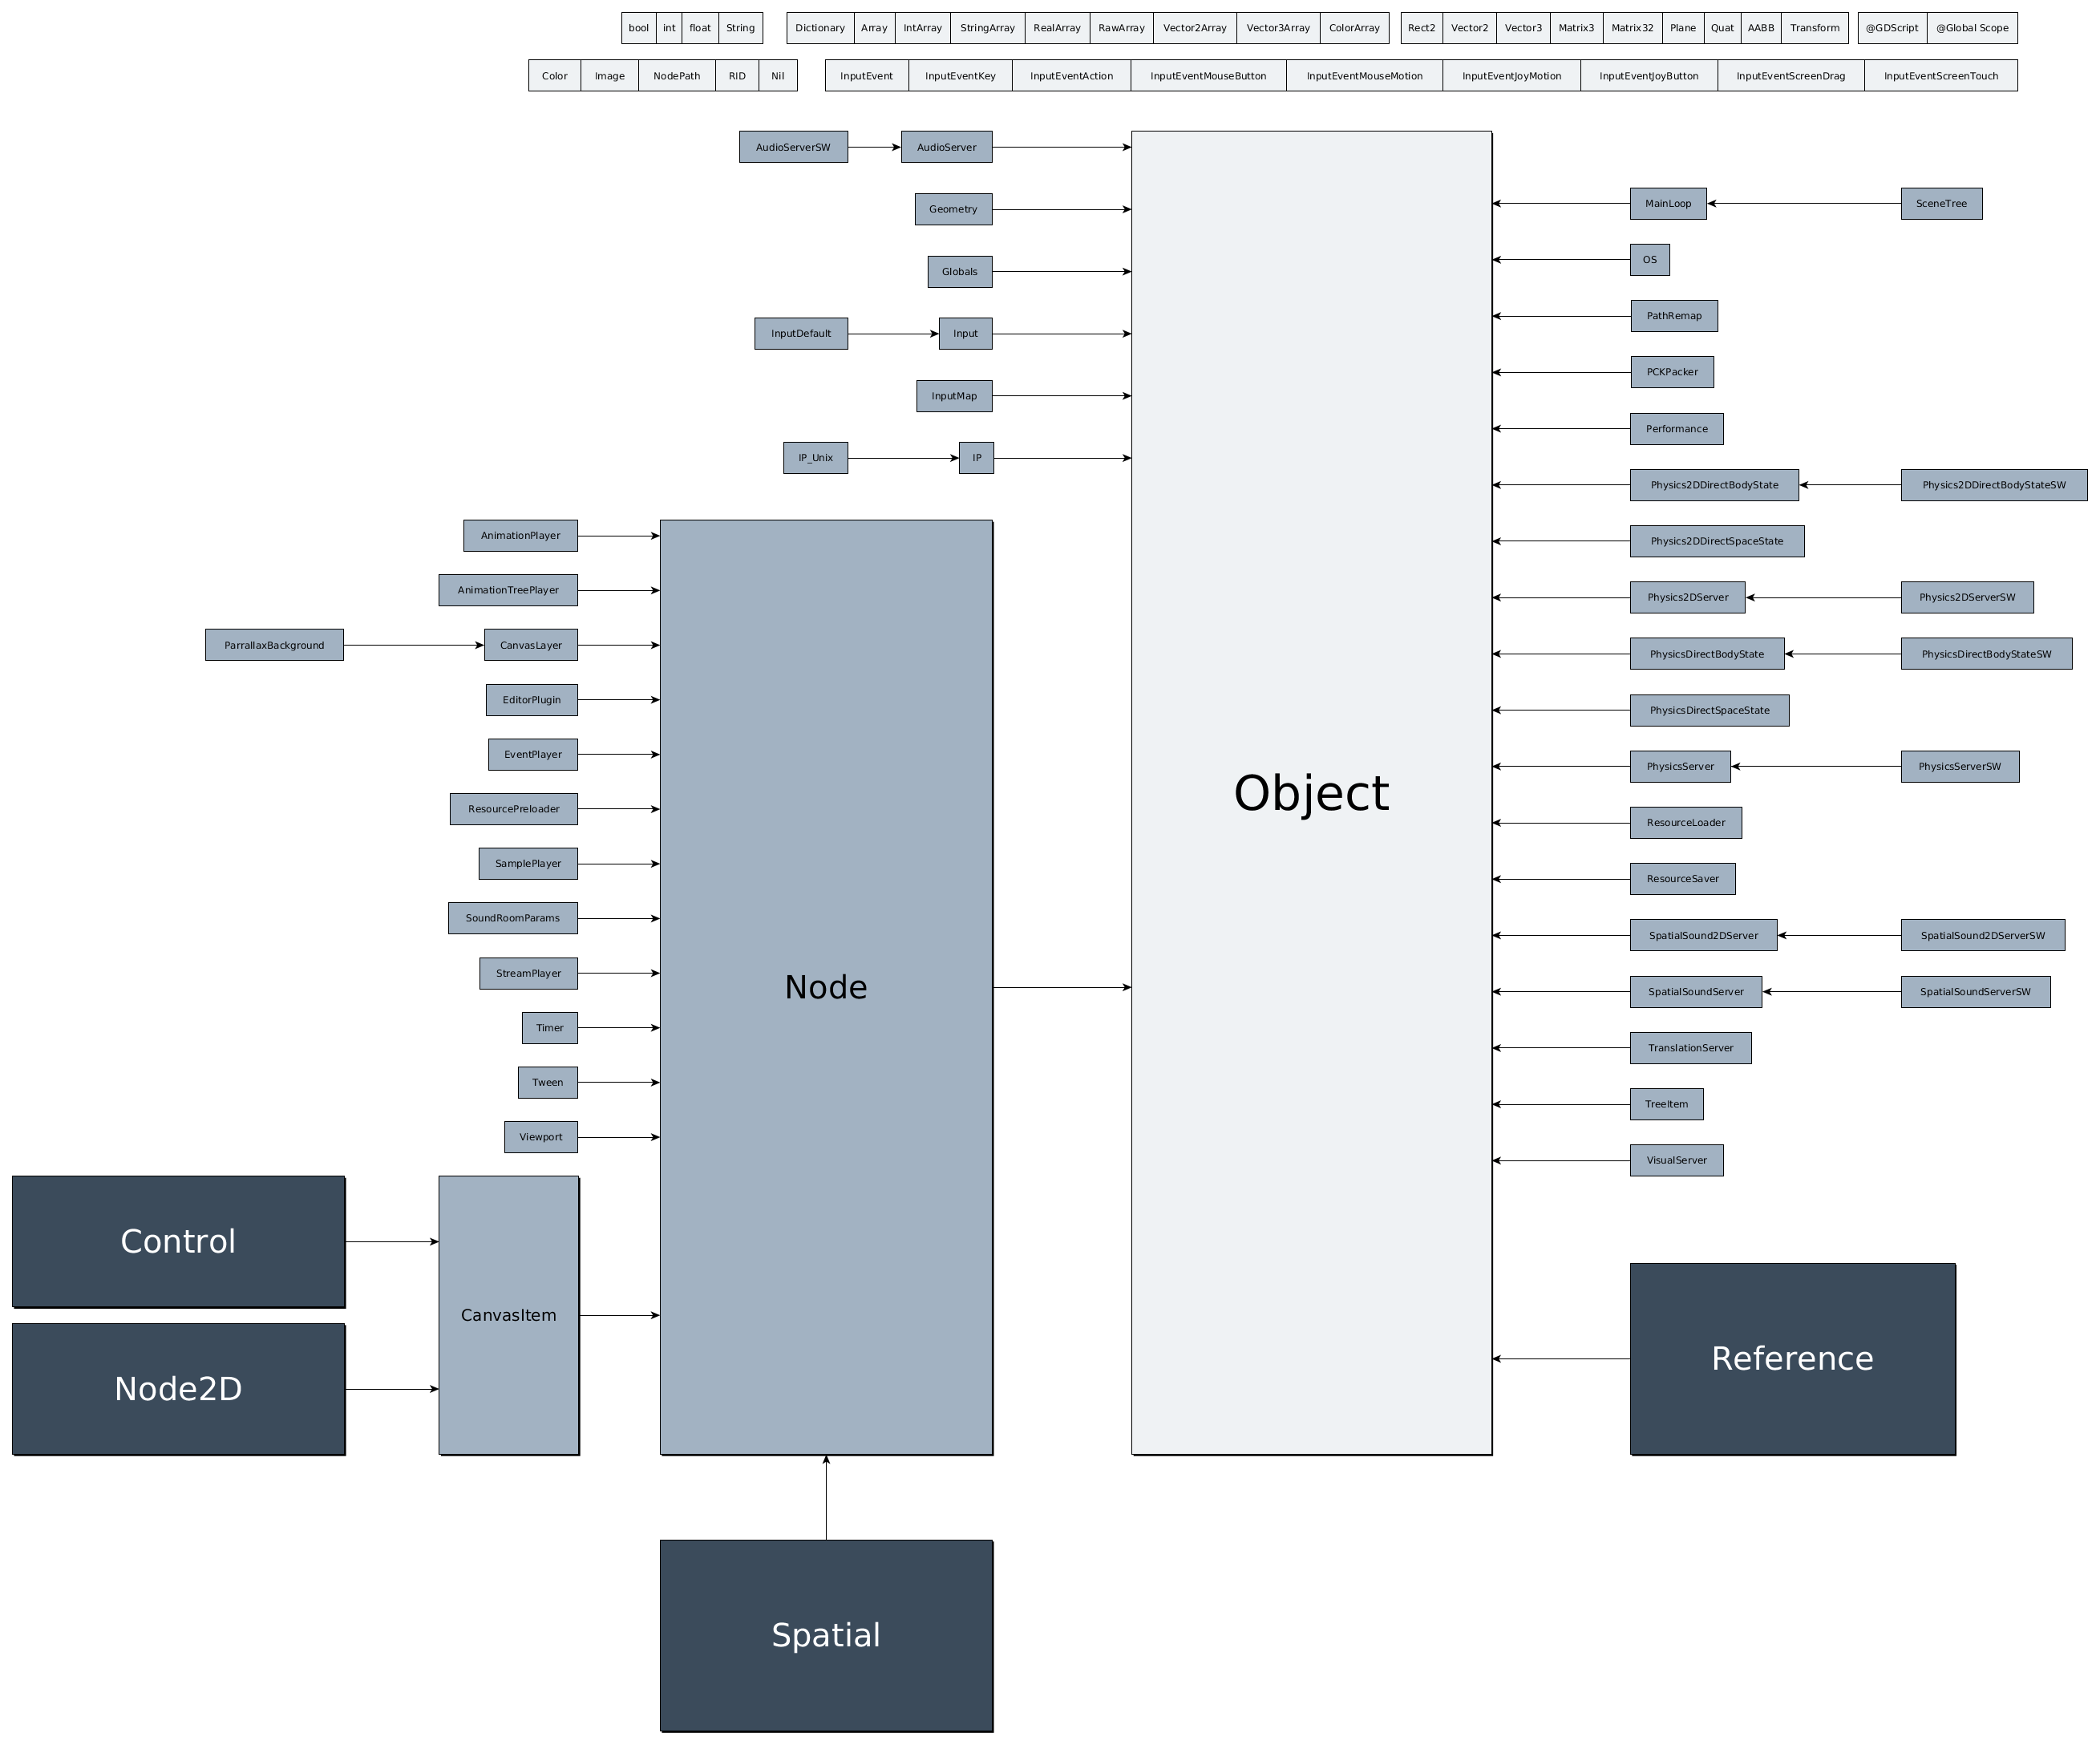
\includegraphics[width=\textwidth]{image/godot-classes.png}
  \caption{Árvore de herança de classes em \textit{Godot} \citep{godotClasses}}
  \label{godotClasses}
\end{figure}

Nas próximas subseções, abordaremos as classes mais importantes, juntamente com as utilidades que trazem para o funcionamento de \textit{Godot}.

% ---------------------------------------------------------------------

\subsection{\textit{Object}}

\textbf{\textit{Object}} (objeto) é a classe base para todos os tipos que não estão já embutidos na \textit{game engine} (como os diferentes tipos de variáveis), conforme fica evidente na figura \ref{godotClasses} apresentada anteriormente.

Algumas de suas características incluem a necessidade de liberar sua memória após o uso e a possibilidade de receber \emph{notificações}, isto é, uma chamada assíncrona, transportando alguma variável, a um de seus métodos.

% ---------------------------------------------------------------------

\subsection{\textit{Reference}}

\textbf{\textit{Reference}} (referência) é uma classe que herda de \textit{Object}. Assim como sua classe pai, ela é mais evidente dentro do código \textit{C++}, pois não aparece diretamente no contexto do editor \textit{Godot}.

Sua principal propriedade está em uma forma de gerenciamento automático de memória, como encontrado na \textit{coleta de lixo} em várias linguagens. Todo \textit{reference} carrega um atributo para contar quantas referências externas possui. Quando não há mais nenhuma, sua memória é automaticamente liberada.

% ---------------------------------------------------------------------

\subsection{\textit{Node}}

Um \textbf{\textit{node}} (nó) é um dos elementos mais básicos para a criação de jogos em \textit{Godot}. Todo \textit{node} herda de \textit{Reference}, e possui um nome, propriedades (que podem ser alteradas/sobrescritas) e um \emph{comportamento}: desenhar um modelo em 3D, mostrar uma interface gráfica, controlar o comportamento de um personagem, etc. \citep{godotNode}. Podem-se criar classes que estendem um tipo de \textit{Node}, atribuindo funcionalidades adicionais a elas.

Em termos práticos, a propriedade mais importante que oferecem é a adição a outros \textit{nodes}, tornando-se filho deles. Com isso, cria-se uma hierarquia de árvore, deixando claro a dependência de funcionalidades.

A seguir, exemplificamos alguns tipos de nós existentes no editor \textit{Godot}.

\begin{itemize}
\item \textbf{\textit{BaseButton}}: Oferece funcionalidades básicas a todos os nós do tipo \textit{button} (botões). Internamente (em \textit{C++}), é implementado como uma classe abstrata.

\item \textbf{\textit{Button}}: É um botão padrão, que pode ser clicado pelo usuário. Estende o nó \textit{BaseButton} (na implementação em \textit{C++}, é uma classe que herda de \textit{BaseButton}).

\item \textbf{\textit{Label}}: Apresenta um texto formatado.

\item \textbf{\textit{Sprite}}: É um \textit{bitmap} bidimensional, tipicamente usado para representar personagens em um jogo 2D.
\end{itemize}

Suponha que desejamos criar um botão clicável, onde está escrito \textit{``Começar Jogo''}. Ao pensarmos que este botão deverá \emph{conter} um texto, a hierarquia de \textit{nodes} fica intuitiva: iremos criar um nó \textit{Button} que possui um filho \textit{Label}. Além disso, desejamos alterar a propriedade de texto deste último para o valor \textit{``Começar Jogo''}.

Teremos uma visão mais prática de nós na seção \ref{cap:color-clutter}, onde criaremos um jogo em \textit{Godot}.

% ---------------------------------------------------------------------

\subsection{\textit{Scene}}

Uma \textbf{\textit{scene}} (cena) é um grupo de \textit{nodes} organizados em uma hierarquia de árvore. Toda cena possui apenas um nó raiz \citep{godotScene}.

Em \textit{Godot}, executar um jogo é equivalente a executar uma ou mais cenas, que podem ser salvas ou carregadas do disco no decorrer do programa. Ressalta-se que, para o jogo começar, uma \textit{scene} deve ser previamente configurada como a inicial, isto é, a primeira a ser executada quando o jogo é iniciado.

A maior vantagem de um \textit{scene}, portanto, está em sua modularização. Ao invés de se criar um jogo grande com uma quantidade enorme de nós em hierarquia, podem-se fazer várias cenas, com uma \emph{instanciando} outra durante a execução. Tal instância é adicionada na árvore da \textit{scene} que fez a chamada. Quando a cena não é mais necessária, ela pode ser salva no disco, se necessário, e retirada da hierarquia.

A figura \ref{sceneInstance} exemplifica um instanciamento genérico de uma cena.

\begin{figure}[H]
  \centering
  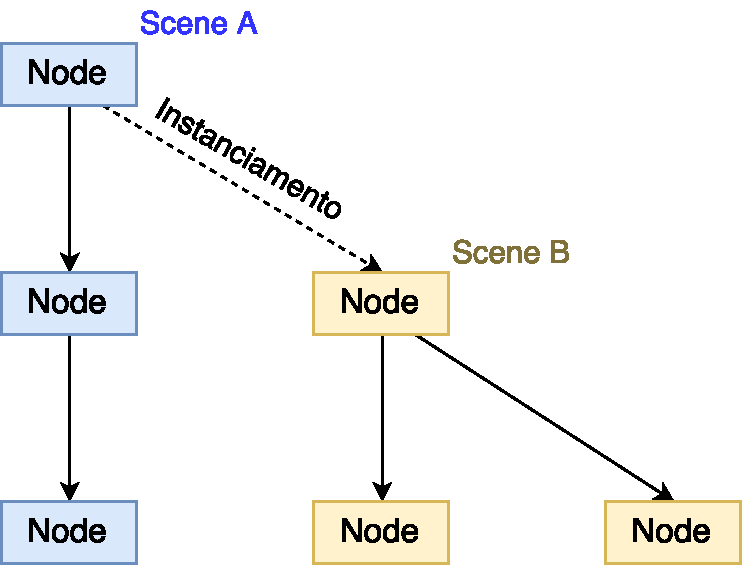
\includegraphics[width=.5\textwidth]{image/scene.pdf}
  \caption{Exemplo de instanciamento de uma \textit{scene} \citep{godotScene}}
  \label{sceneInstance}
\end{figure}

% ---------------------------------------------------------------------

\subsection{\textit{Resource}}

\textbf{\textit{Resources}} (recursos) são outro tipo de dados em \textit{Godot} com uma importância tão grande quanto \textit{nodes}. Todo recurso armazena algum dado, e portanto não realizam uma ação ou processamento por si só \citep{godotResource}.

Uma característica importante de \textit{resources} é que são carregados apenas uma vez do disco. Se um recurso que já está na memória for novamente carregado, será retornado a mesma cópia de antes; em detalhes internos, \textit{Godot} guarda uma referência ao \textit{resource} original.

A classe \textit{Resource} herda de \textit{Reference}, adquirindo sua característica de liberação automática de memória quando não há nenhuma referência à instância.

Exemplos de \textit{resources} incluem:

\begin{itemize}
\item \textbf{\textit{Texture}}: Representa uma textura a ser aplicada em um objeto 2D ou 3D.

\item \textbf{\textit{Font}}: Representa uma fonte a ser usada em um texto, interface gráfica, etc.

\item \textbf{\textit{AudioStream}}: Usado para guardar um fluxo de áudio (uma música a ser tocada no jogo, por exemplo).
\end{itemize}

Exemplificamos, na figura \ref{nodeResource}, alguns \textit{nodes} que tipicamente poderiam usar os \textit{resources} citados.

\begin{figure}[H]
  \centering
  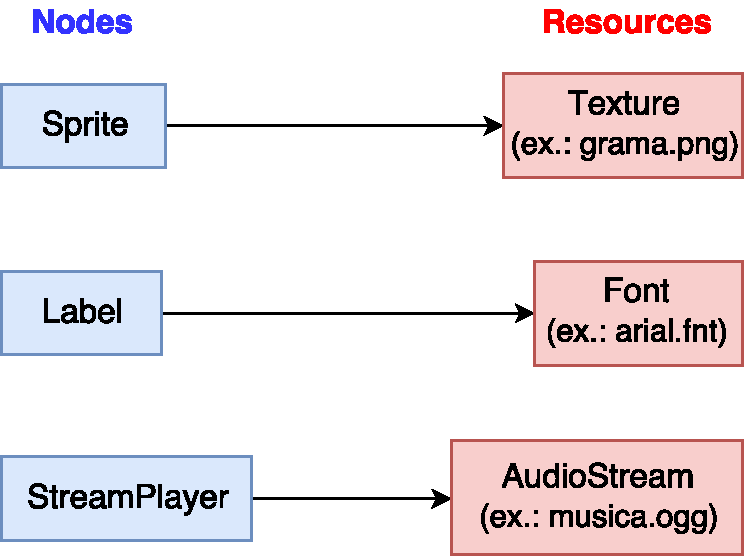
\includegraphics[width=.5\textwidth]{image/resource.pdf}
  \caption{Alguns \textit{resources} e \textit{nodes} que tipicamente os usam \citep{godotResource}}
  \label{nodeResource}
\end{figure}

% ---------------------------------------------------------------------

\subsection{Sistema de arquivos}

Devido ao suporte a diferentes sistemas operacionais, \textit{Godot} viu uma necessidade de criar um padrão interno para gerenciar arquivos em seus projetos (isto é, jogos). Duas convenções foram tomadas:

\begin{itemize}
\item O diretório raiz do projeto é referido como \textbf{\texttt{res://}}. O usuário é encorajado fortemente a utilizar este prefixo ao invés do utilizado em sua plataforma.

\item Caminhos que usem \texttt{res://} devem usar o caractere \texttt{/} para separar diretórios, independentemente do sistema operacional do usuário. Por exemplo: \texttt{res://fontes/arial.fnt}.
\end{itemize}

Por fim, muitos jogos possuem a necessidade de criar, ler, escrever e atualizar arquivos durante sua execução; uma situação comum é guardar o progresso do jogador. Em geral, não é aconselhável criair tais arquivos dentro do diretório do projeto; tal ação é impossível, aliás, se o jogo estiver no formato de um binário fechado.

A solução apresentada por \textit{Godot} foi definir um outro prefixo, \textbf{\texttt{user://}}, que refere-se a algum diretório preestabelecido e externo ao projeto. Em sistemas \textit{Unix}, o caminho tipicamente corresponde a \texttt{\textasciitilde/.godot/app\_userdata}.

% ---------------------------------------------------------------------

\section{\textit{SCons}}

\textit{Godot} pode ser compilado para diversas plataformas; entre elas, citamos Windows, MacOS, Unix, Android, iOS e HTML5. A necessidade de atender a uma variedade tão grande de sistemas operacionais fez com que o projeto escolhesse \textbf{\textit{SCcons}} para simplificar sua compilação \citep{godotScons}. Esta é uma ferramenta de construção de código aberto, como \textit{automake} e \textit{cmake}, mas apresenta algumas vantagens interessantes \citep{scons}:

\begin{itemize}
\item Compilação multiplataforma. Por exemplo, é possível compilar um executável para Windows em um sistema Unix.

\item Todos os arquivos de configuração são \textit{scripts} na linguagem \textit{Python}.

\item Análise de dependências automática para linguagens como \textit{C}, \textit{C++} e \textit{Java}. Não é necessário, por exemplo, listar quais arquivos de código fonte são necessários para compilar o binário final, algo que ocorre em um sistema \textit{Make}.
\end{itemize}

% ---------------------------------------------------------------------

\subsection{Instalação}

\textit{SCons} pode ser instalado pela linha de comando. Em um ambiente Ubuntu, por exemplo, digitaria-se:

\begin{lstlisting}[language=Bash]
$ sudo apt-get install scons
\end{lstlisting}

Também é possível baixar um binário ou o código fonte pelo site \citep{sconsDownload}.

% ---------------------------------------------------------------------

\subsection{Uso em \textit{Godot}}

Para usar o SCons com os \textit{scripts} de configuração em um diretório, basta invocá-lo:

\begin{lstlisting}[language=Bash]
$ scons
\end{lstlisting}

\textit{Godot} oferece alguns argumentos por linha de comando para maior controle sobre a compilação, que usaremos na seção \ref{godotCompile} e no capítulo \ref{cap:color-clutter}. Veja a tabela \ref{sconsParams} para maiores informações.

\begin{table}[H]
\centering

\begin{tabular}{|c|C{.35\textwidth}|L{.4\textwidth}|}
\hline
\textbf{Parâmetro} & \textbf{Significado} & \thead{\textbf{Valores}} \\ \hline

\texttt{p, platform} & Plataforma alvo da compilação &
\makecell[l]{
  Inclui: \\
  \begin{tabular}{@{}ll@{}}
    \texttt{x11} (Unix) & \texttt{javascript} (Web) \\
    \texttt{windows} & \texttt{android} \\
    \texttt{osx} & \texttt{iphone} \\
  \end{tabular}
} \\ \hline

\texttt{bits} & Nº de bits da plataforma alvo &
\makecell[l]{
  \texttt{32} \\
  \texttt{64} \\
  \texttt{default}
} \\ \hline

\texttt{tools} & Deve-se incluir o editor \textit{Godot} no binário? &
\makecell[l]{
  \texttt{yes} \\
  \texttt{no}
} \\ \hline

\texttt{target} & Controla opções de otimização e \textit{debug} &
\makecell[l]{
  \texttt{debug} \\
  \texttt{release\_debug} \\
  \texttt{release}
} \\ \hline

\texttt{j} & Nº de processadores usados para compilação em paralelo &
Um inteiro compatível com o nº de processadores na máquina \\ \hline
\end{tabular}

\caption{Argumentos por linha de comando do \textit{SCons} para \textit{Godot}}
\label{sconsParams}
\end{table}

Algumas explicações devem ser dadas sobre a tabela \ref{sconsParams}. A opção \texttt{default} do parâmetro \texttt{bits} possui grande dependência do sistema operacional em uso: se for Windows ou MacOS, é equivalente a \texttt{32}; se for Unix, assume a mesma quantidade de bits do sistema.

O binário produzido pode ser usado para executar jogos na plataforma para a qual foi criado. A opção \texttt{tools} controla se ele deverá conter, ou não, o editor \textit{Godot}. Executáveis criado com o valor \texttt{no} são chamados de \emph{templates de exportação}, pois são usados para exportar jogos para um determinado sistema operacional.

Por fim, a opção \texttt{target} apresenta três valores possíveis para controlar o uso símbolos de depuração em \textit{C++}, otimização e verificação de erros em tempo de execução (\textit{runtime}). Sintetizamos as características de cada valor na tabela \ref{sconsTarget}.

\begin{table}[H]
\centering

\begin{tabular}{|l|c|c|c|}
\hline
\thead{\textbf{Valor}} & \textbf{Símbolos de depuração} & \textbf{Otimização} & \textbf{Verificação em \textit{runtime}} \\ \hline

\texttt{debug}              &
  {\color{green}\checkmark} &
  {\color{red} x}           &
  {\color{green}\checkmark} \\ \hline

\texttt{debug\_release}     &
  {\color{red} x}           &
  {\color{red} x}           &
  {\color{green}\checkmark} \\ \hline

\texttt{release}            &
  {\color{red} x}           &
  {\color{green}\checkmark} &
  {\color{red} x}           \\ \hline
\end{tabular}

\caption{Valores possíveis do parâmetro \texttt{target} e seu significado}
\label{sconsTarget}
\end{table}

% ---------------------------------------------------------------------

\section{Compilação}
\label{godotCompile}

O código fonte de \textit{Godot} está disponível no \textit{GitHub} \citep{godotRepo}. A criação de um módulo, conforme será visto no capítulo \ref{cap:stt-module}, exige a adição de código à \textit{game engine} e sua recompilação, o que justifica a importância dos passos a seguir.

Antes de começar, verifique se seu sistema \textit{Unix} possui as seguintes dependências:

\begin{itemize}
\item \textit{GCC} (versão 6 ou menor) ou \textit{Clang};
\item \textit{Python} 2.7+ (excluindo-se versões de \textit{Python} 3);
\item \textit{SCons};
\item \texttt{pkg-config};
\item Bibliotecas de desenvolvimento \textit{X11}, \textit{Xcursor}, \textit{Xinerama} e \textit{XRandR};
\item Bibliotecas de desenvolvimento \textit{MesaGL};
\item Bibliotecas de desenvolvimento \textit{ALSA};
\item Bibliotecas de desenvolvimento \textit{PulseAudio};
\item \textit{Freetype};
\item \textit{OpenSSL};
\item \texttt{libudev-dev}.
\end{itemize}

A página de documentação de \textit{Godot} em \citep{godotReq} oferece comandos de terminal para baixar as dependências facilmente nas distribuições \textit{Unix} mais populares. Em \textit{Ubuntu}, por exemplo, faríamos:

\begin{lstlisting}[language=Bash]
$ sudo apt-get install build-essential scons pkg-config libx11-dev \
  libxcursor-dev libxinerama-dev libgl1-mesa-dev libglu-dev \
  libasound2-dev libpulse-dev libfreetype6-dev libssl-dev libudev-dev \
  libxrandr-dev
\end{lstlisting}

Feito isso, siga os passos a seguir para compilar \textit{Godot} na versão 2.1.4.

\begin{enumerate}
\item Clone o repositório da \textit{game engine}.

\begin{lstlisting}[language=Bash]
$ git clone https://github.com/godotengine/godot
\end{lstlisting}

\item Dentro do diretório \texttt{godot/} criado pelo passo anterior, mude para a \textit{tag} corresponde à versão 2.1.4.

\begin{lstlisting}[language=Bash]
$ git checkout 2.1.4-stable
\end{lstlisting}

\item Compile \textit{Godot} através da ferramenta \textit{SCons}; deve levar em torno de 15 minutos.

\begin{lstlisting}[language=Bash]
$ scons p=x11
\end{lstlisting}
\end{enumerate}

% ---------------------------------------------------------------------

\subsection{Verificação}

Se a compilação foi feita com sucesso, um diretório \texttt{bin/} será gerado dentro de \texttt{godot/}. Execute o binário nele contido para abrir o editor \textit{Godot}.

\begin{lstlisting}[language=Bash]
$ ./bin/godot.x11.tools.32  # Em sistema Unix, 32 bits
$ ./bin/godot.x11.tools.64  # Em sistema Unix, 64 bits
\end{lstlisting}

O uso do editor em si será visto no capítulo \ref{cap:color-clutter}, quando criarmos um jogo para demonstrar o módulo de reconhecimento de voz.
